%%%%%%%%%%%%%%%%%%%%%%%%%%%%%%%%%%%%%%%%%%%%%%%%%%%%%%%
%% Bachelor's & Master's Thesis Template             %%
%% Copyleft by Artur M. Brodzki & Piotr Woźniak      %%
%% Covered for Lab/Assigment report by Tymon Żarski  %%
%% Faculty of Electronics and Information Technology %%
%% Warsaw University of Technology, 2019-2020        %%
%%%%%%%%%%%%%%%%%%%%%%%%%%%%%%%%%%%%%%%%%%%%%%%%%%%%%%%

\documentclass[
    left=2.5cm,         % Sadly, generic margin parameter
    right=2.5cm,        % doesnt't work, as it is
    top=2.5cm,          % superseded by more specific
    bottom=3cm,         % left...bottom parameters.
    bindingoffset=6mm,  % Optional binding offset.
    nohyphenation=false % You may turn off hyphenation, if don't like.
]{eiti/eiti-report}

\langpol % Dla języka angielskiego mamy \langeng
\graphicspath{{img/}}             % Katalog z obrazkami.
\addbibresource{bibliografia.bib} % Plik .bib z bibliografią
\usepackage[utf8]{inputenc}
\usepackage[T1]{fontenc}
\usepackage{fourier, erewhon}
\usepackage{geometry}
\usepackage{array, caption, floatrow, tabularx, makecell, booktabs}%
\usepackage{graphicx}
\usepackage{subcaption}
\usepackage{mwe}
\graphicspath{ {img/} }

\captionsetup{labelfont = sc}
\setcellgapes{3pt}

\begin{document}

%--------------------------------------
% Strona tytułowa
%--------------------------------------
\instytut{XXXXXX}
\przedmiot{Wprowadzenie do przetwarzania \\języka naturalnego - projekt}
\specjalnosc{Sztuczna Inteligencja}
\title{
    Transliteracja w tłumaczeniu maszynowym
}
\reportDescription{
    Projekt końcowy
}

\author{Bartosz Cywiński, Łukasz Staniszewski}
\album{304025, 304098}

\prowadzacy{mgr inż. Mateusz Klimaszewski}
\date{\today}
\maketitle

%--------------------------------------
% Spis treści
%--------------------------------------
\tableofcontents

%--------------------------------------
% Rozdziały
%--------------------------------------
\cleardoublepage % Zaczynamy od nieparzystej strony
\pagestyle{headings}

\newpage % Rozdziały zaczynamy od nowej strony
\section{Opis projektu}
Celem projektu jest zbadanie, czy transliteracja ma wpływ na efektywność tłumaczenia maszynowego w przetwarzaniu języka naturalnego. W tym celu wykonane zostało porównanie efektywności tłumaczenia zdań arabskich na angielskie do tłumaczenia tych samych zdań arabskich, ale poddanych wcześniej romanizacji, również na angielski. Ze względu na specjalistyczność słownictwa wykorzystanego w projekcie zamieszczone zostały wyjaśnienia niektórych pojęć:
\begin {enumerate}
    \item \textbf{transliteracja} - konwersja tekstu zapisanego oryginalnie znakami jednego alfabetu z użyciem znaków innego alfabetu, oparta na zasadzie ścisłej odpowiedniości liter (zawsze konkretnemu, jednemu grafemowi wejściowego systemu odpowiada jeden, ten sam grafem z drugiego wyjściowego);
    \item \textbf{romanizacja / latynizacja} - proces transliteracji zakładający, że wyjściowym systemem językowym w procesie jest system opisany przy użyciu alfabetu łacińskiego;
    \item \textbf{korpus} - zbiór tekstów służący do wykonywania badań lingwistycznych i wspomagający metody uczenia maszynowego (w przypadku tego projektu - do tłumaczenia maszynowego); 
\end{enumerate}

\section{Wybrane narzędzia}
Użytym w projekcie językiem programowania (do przetworzenia danych i liczenia metryk) jest Python wraz ze skryptami Bash. Ponadto wykorzystane zostały narzędzia (z dostępnych publicznie bibliotek):
\begin{enumerate}
    \item Preprocessing: \textbf{\href{https://github.com/google/sentencepiece}{SentencePiece}} (tokenizacja), \textbf{\href{https://github.com/CAMeL-Lab/Arabic_ALA-LC_Romanization}{ALA-LC Romanizator}} (romanizacja), \textbf{\href{https://github.com/saffsd/langid.py}{langid}} (wykrywanie języka).
    \item Wykorzystanie i trening modeli - \textbf{\href{https://fairseq.readthedocs.io/en/latest/}{Fairseq}}.
    \item Ocena tłumaczenia: \textbf{\href{https://github.com/mjpost/sacrebleu}{SacreBleu}}, \textbf{\href{https://unbabel.github.io/COMET/html/index.html}{COMET}}.
\end{enumerate}

\section{Źródło danych}
\subsection{Dane treningowe}
Aby modele nie nauczyły się tylko specyficznego stylu pisania, użyte zostały dane z trzech źródeł (wszystkie korpusy są dostępne za darmo na stronie \href{https://opus.nlpl.eu/}{OPUS}). Poniżej przedstawione zostały korpusy, które zostały wykorzystane w projekcie:
\begin{enumerate}
    \item \textbf{CCMatrix} - korpus skonstruowany przez Facebook'a, opisany w \cite{CCmatrix}, składający się z miliardów par zdań w różnych językach. Wartość BLEU dla par zdań arabsko-angielskich mierzona na zbiorze danych składającym się ze zdań wygłaszanych podczas "TED talków"  \cite{Ye2018WordEmbeddings} wynosi 28.7. W projekcie wykorzystano milion par zdań arabsko-angielskich pochodzących z tego zbioru.
    \item \textbf{OpenSubtitles2016} - korpus składający się z napisów do filmów i seriali opisany w \cite{OpenSubtitles}. W projekcie użyto 2 miliony par zdań z wersji korpusu z 2016 roku. Dla par zdań arabsko-angielskich wartość BLEU wynosi 25.34. 
    \item \textbf{News-Commentary v16} - korpus składający się z wpisów informacyjnych z amerykańskich mediów \cite{TIEDEMANN12.463}. W projekcie wykorzystano wszystkie dostępne pary zdań arabsko-angielskie z tego korpusu, ponieważ są one wysokiej jakości, a także jest ich względnie niedużo, bo tylko nieco ponad 83 000 .
\end{enumerate}

\subsection{Dane testowe}
Po analizie dostępnej literatury, zdecydowano, że jako zbiór testowy w projekcie wykorzystany zostanie korpus \textbf{TED2020} \cite{reimers-2020-multilingual-sentence-bert} składający się z transkrypcji popularnych TED-talków - jest to zbiór o wysokiej jakości, więc zastosowanie go do ewaluacji jest miarodajne i pozwala porównać modele z dostępną literaturą \cite{CCmatrix}. 

\section{Przygotowanie danych}

\subsection{Czyszczenie danych i podział}
Zdania z wykorzystywanych korpusach są dostarczone w znacznej większości w odpowiedniej formie (np. bez nadmiarowych znaków). Żeby jednak wyeliminować ewentualny szum w danych odrzucone zostały zdania składające się z mniej niż 3 słów, a także składające się z więcej niż 100 słów. Ponadto wyeliminowane zostały nadmiarowe białe znaki i tagi html. Aby upewnić się, że na wejście modelu trafiają tylko zdania w interesujących językach, przy użyciu pakietu \href{https://github.com/saffsd/langid.py}{langid} wykryte zostały i odrzucone zdania w językach odpowiednio innym od arabskiego i angielskiego. Tak wyczyszczone dane tworzą ostateczne zbiory (nie uwzględniając jeszcze na tym etapie procesu romanizacji). Ostatnim działaniem w tym etapie było wydzielenie ze zbioru treningowego, zbioru walidacyjnego o rozmiarze $10\%$ rozmiaru całego zbioru.  

\subsection{Romanizacja}
Wszystkie przetworzone zdania arabskie zostały poddane transliteracji (przy użyciu narzędzia wspomnianego wcześniej). W wyniku zastosowania konwersji utworzone zostały dodatkowe zbiory danych, na których model będzie zarówno uczony, walidowany jak i testowany. Każde zdanie arabskie znajdujące się w zbiorach dostarczane jest na wejście modelu zaimplementowanego w wykorzystanej bibliotece. Predykcje tego modelu transliterującego (MLE Simple) opierają się na metodzie największej wiarygodności. Model został wytrenowany na wszystkich danych treningowych zawartych w repozytorium biblioteki. Jak przedstawiono w \cite{fadhl2021automatic} wykorzystany model na zbiorze testowym użytym przez autorów publikacji osiąga skuteczność na poziomie $92.2\%$, gdzie w procesie ewaluacji transliteracji nie jest uwzględniana wielkość liter ani interpunkcja.

\subsection{Tokenizacja}
Po zdobyciu wszystkich potrzebnych danych (i ich przetworzeniu), kolejnym etapem była tokenizacja wszystkich zdań (podzielenie zdań na 'wyrazy'). W tym celu dla każdej pary biorącej udział w badaniach: arabski-angielski i arabski po romanizacji-angielski wykonana została następująca sekwencja operacji:
\begin{enumerate}
    \item Wytrenowanie modelu tokenizacji na zbiorze trenującym.
    \item Zakodowanie zdań dla zbioru treningowego, walidacyjnego i testowego. 
\end{enumerate}
Dla obu par systemów jęzkowych zdecydowano się na słowniki o rozmiarach $16000$, wybrano algorytm kodowania \textbf{BPE (Byte Pair Encoding)}, a pokrycie znaków wybrano na poziomie $0.995$ - takie ustawienia pozwoliły na pozbycie się ze słownika znaków niepożądanych takich jak emotki czy pojedyncze znaki z alfabetów innych języków (np. chińskiego), a także na zareprezentowanie bogatego w litery alfabetu arabskiego.

\subsection{Binaryzacja}
Ostatnim elementem niezbędnym do tego, aby można było wykorzystać otrzymane dane, jest ich binaryzacja wraz ze słownikiem otrzymanym w ramach tokenizacji - jest to działanie, którego wymaga użyte w projekcie narzędzie do tłumaczenia maszynowego.

\section{Modele i trening}
    Po zdobyciu przetworzonych danych, eksperymenty rozpoczęto od wytrenowania dwóch modeli tłumaczenia maszynowego - bazowego (dokonującego tłumaczenia z języka arabaskiego na język angielski) oraz poddanego transliteracji (dokonującego tłumaczenia z języka arabskiego zapisanego w alfabecie łacińskim na język angielski). Eksperymenty te wykonano przy użyciu dwóch architektur Sieci Neuronowych: Koder-Dekoder LSTM z mechanizmem Atencji oraz Tiny Transformer.


\begin{table}[h]
  \floatsetup{floatrowsep=qquad, captionskip=4pt}
  \begin{floatrow}[2]
    \makegapedcells
    \ttabbox%
    {\begin{tabularx}{0.45\textwidth}{|c| *{1}{>{\centering\arraybackslash}X|}}
      \hline
      Parametr & Wartość \\
      \hline
      Liczba epok & 24 \\ \hline
      Learning rate & 0.15\\ \hline
      Optymalizator & NAG \\ \hline
      Dropout & 0.2 \\ \hline
      Seed & 0 \\ \hline
      \end{tabularx}}
    {\caption[Hiperparametry dla architektur Tiny Transformer]{Hiperparametry dla architektur Tiny Transformer}
      \label{val1}}
    \hfill%
    \ttabbox%
    {\begin{tabularx}{0.45\textwidth}{|c| *{1}{>{\centering\arraybackslash}X|}}
      \hline
      Parametr & Wartość \\
      \hline
      Liczba epok & 10 \\ \hline
      Learning rate & 0.15\\ \hline
      Optymalizator & NAG \\ \hline
      Dropout & 0.2 \\ \hline
      Seed & 0 \\ \hline
      \end{tabularx}}
    {\caption[Hiperparametry dla architektur LSTM]{Hiperparametry dla architektur LSTM}
      \label{val2}}
  \end{floatrow}
  \vspace*{1cm}
\end{table}%

    \newpage
    W trakcie uczenia każdego z modeli przy użyciu każdej z architektur, spadek straty prezentował się w następujący sposób, gdzie na osi poziomej zaznaczono liczbę kroków, a na pionowej stratę (UWAGA - ze względu na fakt, że modele bez transliteracji były uczone przy użyciu dwukrotnie większych batch'y, badania z nimi związane mają dwukrotnie mniejszą liczbę kroków):
    
    \begin{figure*}[h]
        \centering
        \begin{subfigure}[b]{0.475\textwidth}
            \centering
            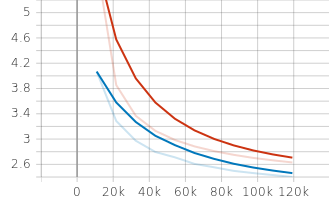
\includegraphics[width=\textwidth]{lstm_basic_loss.png}
            \caption[Network2]%
            {{\small Model bez transliteracji - LSTM}}    
            \label{fig:mean and std of net14}
        \end{subfigure}
        \hfill
        \begin{subfigure}[b]{0.475\textwidth}  
            \centering 
            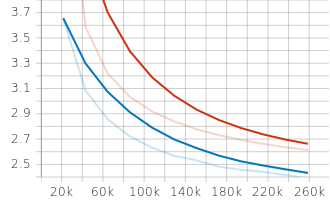
\includegraphics[width=\textwidth]{lstm_romanized_loss.png}
            \caption[]%
            {{\small Model z transliteracją - LSTM}}    
            \label{fig:mean and std of net24}
        \end{subfigure}
        \vskip\baselineskip
        \begin{subfigure}[b]{0.475\textwidth}   
            \centering 
            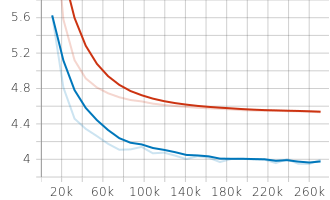
\includegraphics[width=\textwidth]{transformer_basic_loss.png}
            \caption[]%
            {{\small Model bez trainsliteracji - Transformer}}    
            \label{fig:mean and std of net34}
        \end{subfigure}
        \hfill
        \begin{subfigure}[b]{0.475\textwidth}   
            \centering 
            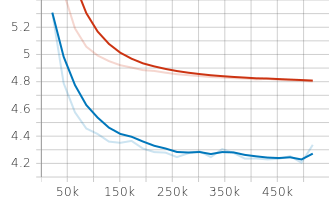
\includegraphics[width=\textwidth]{transformer_romanized_loss.png}
            \caption[]%
            {{\small Model z transliteracją - Transformer}}    
            \label{fig:mean and std of net44}
        \end{subfigure}
        \caption[ The average and standard deviation of critical parameters ]
        {\small Strata obserwowana w trakcie uczenia każdego z modeli przy użyciu każdej architektury, gdzie kolorem pomarańczowym zaznaczona jest strata na zbiorze treningowym, a niebieskim - na zbiorze walidacyjnym. } 
        \label{fig:mean and std of nets}
    \end{figure*}

\section{Ewaluacja}
    
    Po wytrenowaniu obu modeli, zostały one ze sobą porównane pod względem skuteczności. W tym celu skorzystano z dwóch podstawowych automatycznych metryk do tłumaczenia maszynowego: chrF (character F-score) \cite{popovic-2015-chrf}, BLEU \cite{BLEU} oraz COMET \cite{COMET}.
    
    % \begin{center}
\begin{table}[H]
\centering
\footnotesize
\begin{tabular}{ |p{5cm}||p{3cm}|p{3cm}|p{3cm}|  }
    \hline
    \footnotesize{} & \footnotesize{BLEU} & \footnotesize{chrF}&  \footnotesize{COMET} \\
    \hline
     \textbf{LSTM bez transliteracji} & \textbf{21.45}  &  \textbf{45.14}  & \textbf{-0.02} \\
     \hline
     \textbf{LSTM z transliteracją} & 21.15  &  44.50  & -0.35 \\
     \hline
     \textbf{Transformer bez transliteracji} & 12.01  &  33.41  & -0.54 \\
     \hline
     \textbf{Transformer z transliteracją} & 9.87 & 31.08 & -0.85 \\
     \hline
\end{tabular}
\caption{Zmierzone wartości metryk dla każdego przeprowadzonego treningu.}
\label{tab:attr_table}
\end{table}
% \end{center}

Wyraźnie widać, że w obydwu przypadkach Transformer poradził sobie znacznie gorzej od LSTM. Patrząc na wykresy funkcji straty można przypuszczać, że dłuższy trening LSTM prowadziłby do uzyskania jeszcze lepszych wyników, ponieważ krzywa uczenia nie zdążyła się jeszcze do końca wypłaszczyć. Natomiast krzywa uczenia Transformera wypłaszczyła się już po około 12 epokach.\\

Porównując oba modele - ten trenowany na oryginalnym zbiorze danych z tym trenowanym na zbiorze poddanym transliteracji - otrzymano lepsze wyniki dla danych oryginalnych pod względem każdej z metryk. Po metrykach widać bardzo małą różnicę przy okazji LSTM, różnica uwydatnia się tutaj dopiero przy metryce COMET, niemniej jednak w wynikach otrzymanych dla Transformera różnica zaczyna się nieco uwydatniać.\\

\subsection{Analiza predykcji modeli}
Z uwagi na to, że dużo lepsze wyniki osiągnął model LSTM, wnioski i analizy prowadzone zostaną na podstawie predykcji tylko z tego modelu.

Po analizie predykcji modeli na zbiorze testowym widać, że dobrze radzą one sobie z tłumaczniem krótkich wypowiedzi, które składają się maksymalnie z ok. 8 słów.

% \begin{center}
\begin{table}[H]
\centering
\footnotesize
\begin{tabular}{ |p{4cm}|p{10cm}|  }
    \hline
    \textbf{oryginalne zdanie} & I see only specific pictures.\\
     \hline
     \textbf{bez transliteracji} & I see only specific pictures. \\
     \hline
     \textbf{z transliteracją} & I see only specific pictures. \\
     \hline
\end{tabular}
\caption{Oba modele dobrze radzą sobie z tłumaczeniem krótkich zdań.}
\label{tab:attr_table}
\end{table}
% \end{center}

Na podstawie krótkich zdań trudno zauważyć różnicę między modelem uczonym na danych oryginalnych oraz tym poddanym transliteracji, gdyż predykcje często dokładnie pokrywają się.
Jednakże, zbiór testowy składa się również z kilkuzdaniowych wypowiedzi, na których model radzi sobie znacznie gorzej. Na przykładzie dłuższych zdań jest już dostrzegalna różnica w zależności od tego na jakich danych trenowany był model.

% \begin{center}
\begin{table}[H]
\centering
\footnotesize
\begin{tabular}{ |p{4cm}|p{10cm}|  }
    \hline
    \textbf{oryginalne zdanie} & And I had a bit of a wake-up call in Amsterdam: I was there going into the design stores, and mixing with our crowd of designers, and I recognized that a whole lot of stuff pretty much looked the same, and the effect of globalization has had that in our community also.\\
     \hline
     \textbf{bez transliteracji} & I've got a call from sleep in Amsterdam, I've been there going to a designer shop because combined with a crowd of designers, I have realized that many things look like some of them, and that the impact of globalization has appeared in our society, too. \\
     \hline
     \textbf{z transliteracją} & I'm going to sleep in Amsterdam, and the effect of globalization has also emerged in our society. \\
     \hline
\end{tabular}
\caption{Modele gorzej radzą sobie z dłuższymi zdaniami. Widać znaczną różnicę między tłumaczeniami modeli.}
\label{tab:long_sent_table}
\end{table}
% \end{center}
W przedstawionym przypadku w tabeli \ref{tab:long_sent_table} model z transliteracją widocznie pomija tłumaczenie środkowej części oryginalnego zdania, podczas gdy model uczony na oryginalnych danych stara się przynajmniej przetłumaczyć zdanie. Przedstawione powyżej tłumaczenie modelu uczonym na danych bez transliteracji całkiem dobrze oddaje sens zdania, zawiera jednak wiele błędów gramatycznych. Zauważalna jest też zamiana słów w tłumaczeniu na synomimy słów użytych oryginalnie, co zostało przedstawione w tabeli \ref{tab:adjective_table}. Jest to częsty przypadek w predykcjach obu modeli.

% \begin{center}
\begin{table}[H]
\centering
\footnotesize
\begin{tabular}{ |p{4cm}|p{10cm}|  }
    \hline
    \textbf{oryginalne zdanie} & That's a lovely idea.\\
     \hline
     \textbf{bez transliteracji} & That's a nice idea. \\
     \hline
     \textbf{z transliteracją} & That's a beautiful idea. \\
     \hline
\end{tabular}
\caption{Modele zmieniają słowa w zdaniach na synonimy.}
\label{tab:adjective_table}
\end{table}
% \end{center}


Ciekawym porównaniem predykcji jest też ten przedstawiony poniżej w tabeli \ref{tab:numeral_table}. Można tu zauważyć, że mimo praktycznie identycznych predykcji obu modeli inaczej przedstawiona jest godzina - w jednym przypadku jest ona liczbą a w drugim słowem. W zasadzie ciężko jednoznacznie określić, które z tłumaczeń jest poprawniejsze. Z jednej strony model bez transliteracji w swojej predykcji dał słowo, tak samo jak było to w zdaniu oryginalnym. Z drugiej strony model ten niejako pomija człon \textquotesingle \textquotesingle o\textquotesingle clock\textquotesingle\textquotesingle  stanowiący o równej godzinie, a model z transliteracją wyraża to dokładnie w postaci liczby.
% \begin{center}
\begin{table}[H]
\centering
\footnotesize
\begin{tabular}{ |p{4cm}|p{10cm}|  }
    \hline
    \textbf{oryginalne zdanie} & They worked until four o'clock in the morning.\\
     \hline
     \textbf{bez transliteracji} & Keep working till four in the morning. \\
     \hline
     \textbf{z transliteracją} & Keep working till 4:00 in the morning. \\
     \hline
\end{tabular}
\caption{Modele w różny sposób tłumaczą godzinę.}
\label{tab:numeral_table}
\end{table}
% \end{center}

Warto również zwrócić uwagę na to jak modele radzą sobie ze zdaniami podrzędnymi w zdaniach. Przykładowo, gramatycznie wtrącenie w zdaniu jest łatwiejsze do uzyskania przez model nie poddany transliteracji co pokazano w tabeli \ref{tab:insertion}.
% \begin{center}
\begin{table}[H]
\centering
\footnotesize
\begin{tabular}{ |p{4cm}|p{10cm}|  }
    \hline
    \textbf{oryginalne zdanie} & Now it's 0.5 -- even worse than that in America -- showing us the income inequality.\\
     \hline
     \textbf{bez transliteracji} & Now 0.5 – even worse than that in America -- we're building inequality in income. \\
     \hline
     \textbf{z transliteracją} &  Now 0.5-even it is worse in America — we have not equal income inequality. \\
     \hline
\end{tabular}
\caption{Modele w różny sposób tłumaczą godzinę.}
\label{tab:insertion}
\end{table}
% \end{center}

\newpage

\section{Wnioski i podsumowanie}
Jedną z hipotez dlaczego otrzymane zostały lepsze wyniki dla oryginalnych danych jest to, że w procesie transliteracji tracona jest nieco dokładność - w końcu użyte w tym projekcie narzędzie osiąga $90\%$ skuteczności. Transliteracja nieidealnym narzędziem może powodować stratę informacji, co może mieć wpływ na różnicę w wynikach obu modeli, skoro drugi z nich korzysta z oryginalnych danych.\\


Wytrenowane w ramach projektu modele charakteryzują się tym, że potrafią wydobyć sens z tłumaczonego zdania, natomiast przy okazji wyniki translacji są bogate w liczne błędy gramatyczne. Wśród predykcji można zauważyć również zdolność modeli do upraszczania zdań, szczególnie w przypadku przymiotników, gdzie modele preferują przykładowo słowo straszny od słów przerażający i koszmarny. W trakcie analizowania wyników zauważono liczne błędy w predykcjach związane z zaimkami - jest to najprawdopodobniej związane z charakterystyką języka arabskiego, gdzie często w zdaniach pomijany jest podmiot.\\


W \cite{CCmatrix}, gdzie opisano konstruowanie korpusu CCMatrix, dla ewaluacji powstałego zbioru wytrenowano system tłumaczenia maszynowego na powstałym zbiorze, a następnie dokonano ewaluacji na tym samym zbiorze testowym, który został użyty w naszym projekcie. Dlatego też, wyniki otrzymane w artykule mogą posłużyć jako wyniki referencyjne w tym projekcie. Jak już wcześniej zostało to wspomniane, w referencyjnym rozwiązaniu zmierzona metryka BLEU wyniosła 28.7. Najlepszą wartość metryki BLEU w tym projekcie wystąpiła dla LSTM uczonego na zbiorze bez transliteracji i wyniosła ona 21.45. Zważając na to, że rozwiązanie referencyjne trenowane było na zbiorze 6.5 miliona zdań (ponad dwa razy większym od naszego), a także wybrana w tym projekcie architektura sieci neuronowej - Autokoder z Atencją - nie stanowi state-of-art w tłumaczeniu maszynowym, wyniki można uznać za zadowalające.

\clearpage
\printbibliography
\end{document}